\title[JASA/draft]{Real-time Acoustic Ray Range Estimation for Underwater Vehicle Navigation}
\author{EeShan C. Bhatt}
\email{ebhatt@whoi.edu}
\affiliation{MIT-WHOI Joint Program in Oceanography/Applied Ocean Science \& Engineering, Cambridge and Woods Hole, MA, USA}
\affiliation{Department of Mechanical Engineering, Massachusetts Institute of Technology, Cambridge, MA}
\author{Oscar Viquez}
\affiliation{Department of Mechanical Engineering, Massachusetts Institute of Technology, Cambridge, MA}
\author{Bradli Howard}
\affiliation{MIT-WHOI Joint Program in Oceanography/Applied Ocean Science \& Engineering, Cambridge and Woods Hole, MA, USA}
\affiliation{Department of Mechanical Engineering, Massachusetts Institute of Technology, Cambridge, MA}
\author{Henrik Schmidt}
\email{henrik@mit.edu}
\affiliation{Department of Mechanical Engineering, Massachusetts Institute of Technology, Cambridge, MA}

% \author{Author Four}
% \email{author.four@university.edu}
% \affiliation{Department2,  University2, City, State ZipCode, Country}

\preprint{Bhatt, JASA}   %  if you want want this message to appear in upper right corner of title page

\date{\today}

\begin{abstract}
Almost all underwater navigation paradigms rely on the conversion of recorded travel time into range to compute a trilateration solution. For real-time navigation, this conversion is treated deterministically. For positioning in post-processing, more computationally and/or labor intensive modeling methods are often employed to reduce the uncertainty driven by multipath arrivals. For an autonomous underwater vehicle deployment in March 2020 in the Beaufort Sea, the total under-ice environment and complex acoustic propagation via the Beaufort Lens necessitated the real-time integration of model-based data processing. An embedded, stochastic, ray-based prediction of the horizontal group velocity achieved a ranging mean absolute error of 11 m compared to GPS-aided beacon-to-beacon communication events. In post-processing, a multipath adjustment achieved ranging performance that rivals GPS. To our knowledge, these results are the first field experiment to demonstrate a real-time, physics-based model to constrain ranging error in underwater navigation.
\end{abstract}

%% pacs numbers not used

\maketitle

% =========================================================================== %
% =========================================================================== %

\section{\label{sec:1} Introduction}

The paper is organized as follows: Section~\ref{sec:2} presents the physical
experimental setup and data processing simplifications; Section~\ref{sec:3} presents key results for group velocity predictions and range estimations; Section~\ref{sec:4} closes with a discussion.

% =========================================================================== %
% =========================================================================== %
\section{\label{sec:2} Methods}

The operational solution for ICEX20 relied on an Integrated Communication and Navigation Network (ICNN) \citep{schneider_self-adapting_2020,randeni_construction_2020,randeni_high-resolution_2021}.
The ICNN was initially developed via numerous virtual experiments, to push the boundaries of algorithms and interfaces between different hardware components.
The simulation approach is a necessary testbed for robustness and produces better results than post-processing previous field data, as that restricts mission configurations to the data taken, which can hamper troubleshooting in the field.
The simulation capabilities are largely physics-driven with a modular system of systems approach: an environmental simulator with sub-components for the ocean, Arctic ice, and ocean acoustics; a vehicle simulator with sub-components for vehicle dynamics and navigation; a topside hardware simulator and acoustic communications simulator, both with a software and hardware-in-the-loop version \citep{schneider_netsim_2018}.
The virtual environment similarly emulates the interfaces between the real components to test the entire software pipeline.
Both simulation capabilities are integral to mission success.

\subsection{Operational paradigm on the ice}

The ICNN is comprised of four ice buoys, loosely in a rectangle, roughly 2 km away from a central ice camp with a topside computer, as shown in Fig.~\ref{fig:icnnOverview}.

\begin{figure}[h!]
	\centering
	\includegraphics[width=\reprintcolumnwidth]{figs/ICNN_Overview}
	\label{fig:icnnOverview}
	\caption{CAPTION}
\end{figure}

Each ice buoy is outfitted with a WHOI Micro-Modem \citep{singh_underwater_2006}, with a four-element receiver array and a single transmitter, and one-tenth of a millisecond resolution.
The receiving and transmitting elements were split between shallow and deep depths (30 and 90 m, respectively) to provide better coverage due to the acoustic shadow zone in the Beaufort Lens.
The buoys do not encompass the full operating range of the vehicle but are positioned to minimize overlap in trilateration for spherical positioning\citep{deffenbaugh_relationship_1996}.

Vehicle missions in any underwater environment, but especially acoustically complex ones, must balance competing uses of the acoustic channel.
Thus this network uses a single synchronized digital communication packet to provide both tracking and data to the operator.
The ICNN operational paradigm is as follows:
\begin{enumerate}
\item The AUV, running an ice-tracking DVL and an onboard hydrodynamic model, broadcasts its perceived location on a scheduled, time-synchronized message via WHOI Micro-Modem
\item Four ice buoys, each outfitted with a WHOI Micro-Modem, receive messages from the AUV and send that information over freewave radio to a Topside computer
\item The topside computer converts travel times into range estimates using a stochastic embedded prediction of the horizontal group velocity via BELLHOP ray tracing code \citep{porter_bellhop_2011}
\item The topside computer calculates a new position by trilaterating the range estimates
\item The position differential is broadcast to the vehicle to update its navigation solution
\end{enumerate}

This paper specifically addresses the third step\textemdash the topside computer's conversion of travel time into range, which underpins the trilateration in the ICNN, and is an often overlooked element of any underwater acoustic navigation system.
The results accordingly focus on validating acoustic range estimates from communication events between GPS-tracked beacons.
This ``modem experiment'' was conducted while the vehicle was still being prepped to go under the ice.

\subsection{Modem experiment design}

Because the navigation solution on the vehicle, during a mission, can only be evaluated on the basis of the error estimates sent, a sister experiment for validating the real-time ranging approach was implemented.
The ice buoy modems were run as ``virtual vehicles'' at a given depth and would transmit to all other ice buoys.
The internal sound speed estimate was then toggled using a handful of weights applied to a basis function representation of the sound speed.
This trial was configured for as many ice buoy modems as possible, with each experiment running for roughly an hour between the two sound speed modalities.
There are three important engineering choices in the ICNN network to contextualize this dataset:
\begin{enumerate}
\item Each modem buoy only has one transmit depth layer (30 or 90 m)
\item The transmit and receive layers are independent
\item At any given time, the receive depth layers are the same across all four ice buoys
\end{enumerate}

The design enables a self-adapting network to transmit and receive at the optimal depth to maintain contact with the AUV \citep{schneider_self-adapting_2020}.
This adaptivity was not used during the modem experiment but was instead toggled manually.
Given the complexity of the ICNN system, this experiment did not collect an exhaustive set of data across all buoy, source depth, receive layer, and sound speed combinations, as this time was also used to verify and resolve any hardware issues in the modems themselves.

Importantly, only one modem at a time could run the vehicle behavior to trigger group velocity calculations; other modems that were transmitting simultaneously recorded events as modems, not as vehicles.

The dataset introduced in this thesis has parallel physical and virtual layers; given the small operational scale, on the order of kilometers, and a singular SSP, both layers are projected into a range independent coordinate system for ease of comparison.

\subsubsection{Physical layer}
The physical layer, i.e. the physical link through the real ocean, describes the beacon to beacon communication events through the real water column; it covers all source depths (20, 30, and 90 m) and both receive layers (30 and 90 m), where the surface expressions of the beacons are tracked by GPS. Events are sorted by source depth and sound speed profile given that this is the dominating factor for the location and span of the shadow zone compared to any temporal or spatial scales of variability.


\begin{figure}[h!]
  \centering
  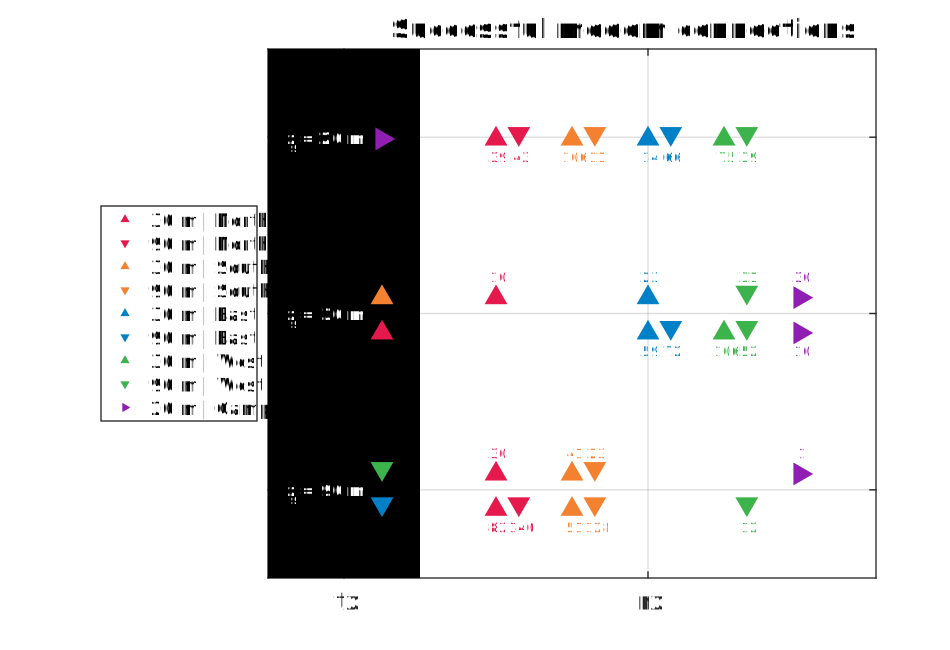
\includegraphics[width=.50\textwidth]{figs/modem-chart.pdf} \hfill
  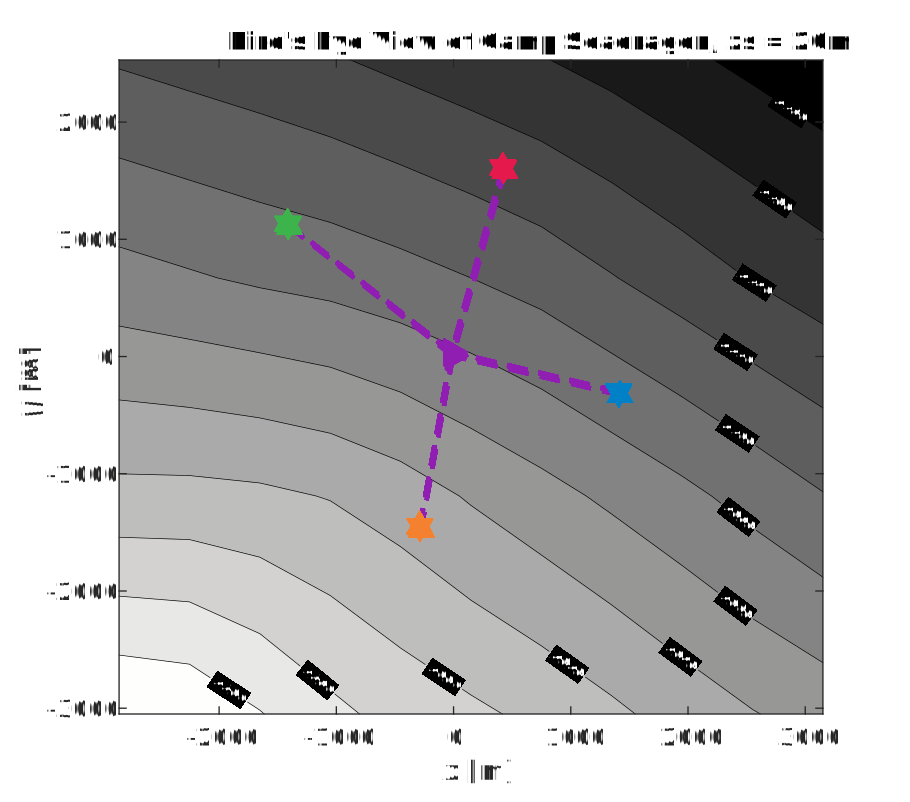
\includegraphics[width=.48\textwidth]{figs/zs20-birdseye.pdf} \\
  \vspace{1em}
  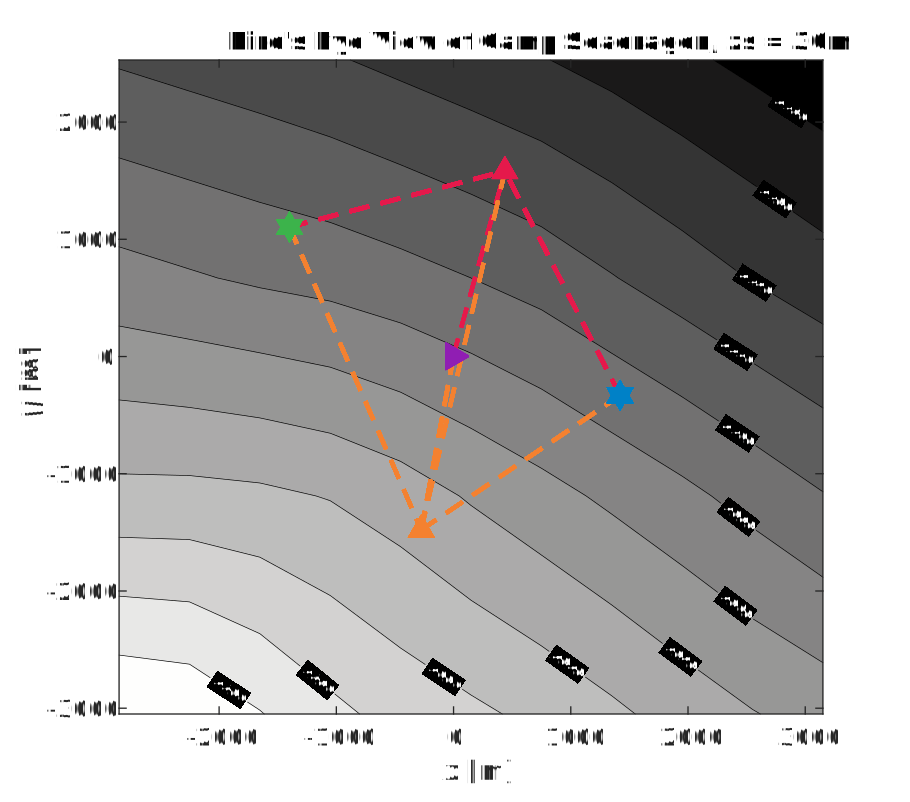
\includegraphics[width=.48\textwidth]{figs/zs30-birdseye.pdf} \hfill
  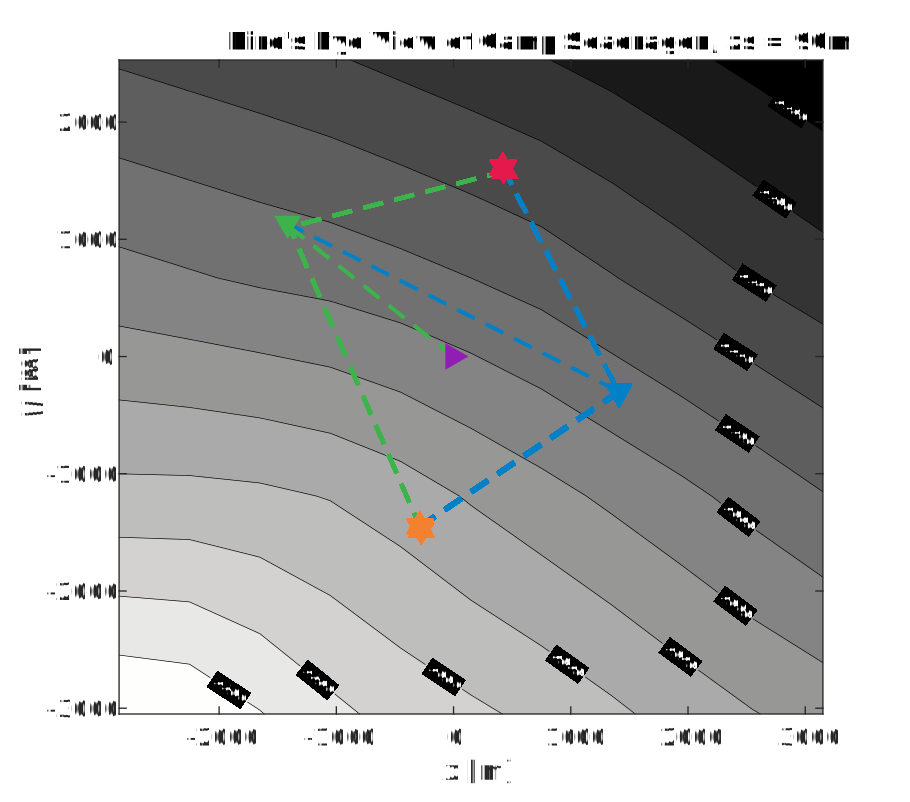
\includegraphics[width=.48\textwidth]{figs/zs90-birdseye.pdf} \\
  \caption{An overview of the modem experiment by source and receiver depth and position. Subfigure (a) shows a chart of the successful events between source and receiver depth. The black column on the left, $tx$, shows the source depth, $z_s$. The column on the right, $rx$, shows the receivers with the amount of good contacts. The orientation of the triangles\textemdash sideways, upwards, and downwards\textemdash corresponds to depths of 20, 30, and 90 m. Subfigures (b-d) correspond to receiver depths of 20, 30, and 90 m, respectively. Camp Seadragon, demarcated by the purple triangle, is situated just north of the continental shelf.}
  \label{fig:overview}
  \end{figure}

\clearpage

\subsubsection{Virtual layer}
The virtual layer describes the BELLHOP simulations for each communication event in the physical layer, where a handful of weights applied to a basis function representation can reconstitute any number of candidate SSPs \citep{bhatt_embedded_2021}.
The SSP is the only configurable input to the group velocity prediction.

During ICEX20, the SSP was toggled between the historical``baseline'' and a ``weighted'' estimate based on a CTD, i.e. an optimal set of weights chosen by a human decision maker via an interactive Tactical Decision Aid framework \citep{bhatt_embedded_2021}.
For the post-processing analysis, we add the SSP from HYCOM for comparison, to mirror the information available on a submarine\textemdash modeled data, historical data, and in situ data.
This order corresponds to increasing ducted conditions of the Beaufort Lens.

Fig. \ref{fig:raytrace-zs30} shows eigenrays in a range independent coordinate system for all three sound speed environments for a source depth of 30 m.
It is important to note that BELLHOP produces an abundance of eigenrays; the ones displayed here are chosen by travel time proximity to the recorded data.
An important pattern is the increased complexity in multipath as ducted conditions increase.

\begin{figure}[h!]
  \centering
  \includegraphics[width=\reprintcolumnwidth]{figs/raytrace-3env-zs-30.pdf}
  \caption{Eigenrays for beacon to beacon events for each nominal source depth of 30 m. The beacons are highlighted in color/marker coding in figure \ref{fig:overview}. The eigenrays are curated from BELLHOP by travel time proximity and are traced in the representative colors over a total ray fan in gray.}
  \label{fig:raytrace-zs30}
  \end{figure}

\FloatBarrier
\subsection{Group velocity prediction methods}

The variation of horizontal group velocity from any source-receiver pair is the fundamental challenge to implement GPS-like navigation in an LBL navigation paradigm, especially in an acoustically complex propagation environment.
The use of the acoustic modem network for tracking relies on the accurate estimates of travel times between the submerged platform and range modems, supported by clock synchronization and a pre-determined scheduling of acoustic events.
For the Beaufort Lens, the strong multipath effects make it virtually impossible to deterministically predict the modem triggering time.

\subsubsection{Minimal bounce criteria}
Instead, for each individual node $i$, an embedded stochastic tracking framework is used to provide a running estimate of the horizontal group velocity $u_{i,j}$ for the conversion from travel time to range from modem $j$, with the ultimate goal of matching the naive group velocity, i.e. the GPS-recorded distance between two nodes divided by the modem-recorded one way travel time between them. 

In the ICEX20 configuration, the acoustic tracking is running on the topside computer, which controls the integrated communication and navigation range.
Here we assume that the group velocities $u_{i,j}$ are smoothly varying over the course of a vehicle mission, i.e., with respect to range, mission time, and the frequency of updates relative to vehicle motion. 
The group velocity is continuously tracked using predictions from the \textit{Virtual Ocean} infrastructure.

When the topside tracking framework receives a modem message, with a time delay, $\Delta t$, from one of the range modems, it will request a new estimate of the group velocity and its associated uncertainty.
The group velocity estimate is found using the extrapolated navigation for range, $\hat{r}$, and an impulse response estimate received in the form of ray travel times $dt_{j}$ and amplitudes $a_{j}$ for that range and depth.

The initial call to BELLHOP is over a sparse, dynamically created depth and range grid, of which the plane wave approximation is used to bring the ray to the range and depth posited by the onboard tracking solution.
Using only the $N_0$ rays with neither surface nor bottom bounces, it will then estimate the current group velocity $u$ from a power weighted average of the ray travel times,
\begin{equation}
u = \frac{\hat{r} \sum_{n=1}^{N_{0}} a_{n}^{2}}{\sum_{n=1}^{N_{0}} dt_{n}a_{n}^{2}} ~, 
\end{equation}
and the associated weighted standard deviation,
\begin{equation}
\sigma_{u} \simeq \sqrt{\frac {\sum_{n=1}^{N_{0}} (dt_{n}-\hat{r}/u)^{2}a_{n}^{2}}{ \sum_{n=1}^{N_{0}} a_{n}^{2}} } \frac{u^{2}}{\hat{r}}
\end{equation}
If no direct paths exist, i.e. $N_{0}=0$, then the group velocity is computed using the same algorithm for the ray arrivals with one bounce, and so on.

Finally, the psuedorange is calculated simply as
\begin{equation}
r_{i,j} = u_{i,j} \Delta t_{i,j} 
\end{equation}

This stochastic method for group velocity calculation can run in real-time, appearing to be orders of magnitude faster than general post-processing methods which seek to determine the specific ray itself that best matches a prominent indicator from the arrival structure.
The method assumes direct path arrival, where multipath over the shallow receiver depth is trivial for the group velocity calculation; thus we call it the minimal bounce criteria (MBC).
The BELLHOP simulation that runs this calculation uses 3600 rays with launch angle fan of -60 to 60 degrees.
However, this high density of launch angles creates a greedy estimator of direct path eigenrays, and this simulation pipeline almost always guarantees a direct path found.
The MBC improves upon a deterministic estimate in that it considers the ray path, travel time, and amplitude to predict a realistic group velocity.

\subsubsection{Nearest Bounce Criteria}

As shown in the eigenray traces, an acoustic arrival does not always take the direct path from source to the receiver, and the path it takes is extremely dependent on the sound speed profile.
Often, BELLHOP will produce a number of arrivals resulting from multiple propagation paths for any source-receiver pair.
The suggested algorithm, the nearest bounce criteria (NBC), is only a slight modification from the minimal bounce criteria, and includes multipath as a new dimension of information with negligible additional computation.

Given a running estimate for the horizontal group velocity $u_{i,j}$ between nodes $i$ and $j$, the navigation system has an extrapolated value for range, $\hat{r}$, in the virtual layer, and a recorded travel time, $\Delta t_{i,j}$, in the physical layer.
Instead of using only the $N_0$ rays with neither surface nor bottom bounces to estimate group velocity, we solve for the power weighted average of the ray travel time for the $N_k$ rays with $k$ bounces,
\begin{equation}
t_k = \frac{\sum_{n=1}^{N_{k}} dt_{n}a_{n}^{2}}{\sum_{n=1}^{N_{k}} a_{n}^{2}} ~, 
\end{equation}
find the nearest matching power weighted average to recorded travel time,
\begin{equation}
t_{i,j,k} = \min_{k=0,1,2,...} \left| t_k - \Delta t_{i,j} \right|
\end{equation}
predict a group velocity,
\begin{equation}
u_{i,j} = \dfrac{\hat{r}}{t_{i,j,k}}
\end{equation}
and estimate the range as was done previously.
\begin{equation}
r_{i,j} = u_{i,j}\Delta t_{i,j}
\end{equation}

This method selects a different group velocity based on the multipath arrival structure, as the expected arrival is not always the first arrival and could even be masked by noise or blocked temporarily \citep{deffenbaugh_acoustic_1996}.

% =========================================================================== %
% =========================================================================== %

\FloatBarrier
\section{\label{sec:4} Real-time psuedorange results}

The modem experiment generated 811 beacon to beacon communication events with their own real-time NBC group velocity predictions.
As expected, the algorithm is generally overestimating range as it resolves a direct path that does not represent the actual arrival.
This section examines the absolute range error between the psuedorange and the GPS derived range with the caveat that the data collected is fairly asymmetrical across source depths and sound speed conditions.

\begin{table}[h!]
\renewcommand{\arraystretch}{1.5}
\centering
\begin{tabular}{r|ccccc}
SSP & Count & Mean [m] & Median [m] & STD [m] & Max [m] \\ \hline
Baseline & 243 & 11.38 & 11.96 & 4.23 & 23.95 \\ 
Chosen weights & 568 & 11.36 & 11.40 & 8.12 & 26.0 \\
\end{tabular}
\caption[Range estimation error for \textit{in situ} events]{The range estimation error for \textit{in situ} events. The error here is presented as the absolute, not directional, error.}
\label{tab:rangeErrorInSitu}
\end{table}

Table \ref{tab:rangeErrorInSitu} breaks down the number of events, mean, median, standard deviation, and maximum absolute range error for the \textit{in situ} calculations.
The mean and median for both sound speeds are similar on the order of centimeters; the chosen weights show a maximum greater than that of baseline, but it is from a OWTT event that has no comparison in the baseline data set.
The overarching statistical results show that both sound speed environments, given the smaller operational scales and shallow depths, are accurate enough to approximate the group velocity structure given a local grid.
Of course, these statistics obscure the relationship between range error and range (or OWTT as the proxy for range).
Analysis shows that where there is overlap in range between sound speed conditions, the range error difference is no more than a few meters.
This is likely driven by the prominence of the duct.

Where there is overlap in the physical layer, i.e. in OWTT, the range error driven by the two virtual layers is no more than a few meters.
This is best demonstrated by all source and receiver depth pairings, except for a source at 30 m and a receiver at 90 m, where the baseline is clearly visibly closer to no range error than the weighted environment.
This may be driven by the prominence of the duct, but it is certainly occluded by the order of magnitude difference between the number of events in each virtual layer.

\FloatBarrier
\section{\label{sec:5} Post-processing psuedorange results}

Due to the operational constraint of only one modem running the vehicle behavior at a time, the previous analysis has looked at 811 total beacon to beacon events, where 243 use the baseline SSP and 568 use the weighted SSP.
While overall statistics are presented, and individual events are compared for the same SSP between the two algorithms, the events themselves are not equally distributed with respect to depth, range, and sound speed status.

The analysis is separated by source depth, and where possible, receiver depth, as the group velocities across source and receiver depths may be different.

There are 1242 total beacon to beacon events in the modem experiment that would have been accepted by the ICNN for real-time ranging and navigation had the vehicle behavior been running on all modems.
The value for the extrapolated range, $\hat{r}$, is only tracked when the modem runs the vehicle behavior; thus we replace $\hat{r}$ with the GPS-tracked range for all modem events.
Naturally, because $\hat{r}$ converges to the correct solution, a comparison of $\hat{r}$ with the GPS-tracked range shows a normal, zero-centered distribution within the bounds of GPS drift.
The analysis here therefore seeds ``omniscient'' knowledge of the range and leverages the post-processing pipeline to more thoroughly evaluate the acoustic range estimate for all modem events, with all three sound speed sources, and both group velocity criterion.
Thus, the results in this section evaluate the utility of the algorithms and sound speed sources, divorced from their role in the ICNN.
We first compare the post-processing results between the two algorithms, and then take a step-by-step approach to examine how the nearest bounce algorithm works in more detail.

\FloatBarrier
\subsection{Group velocity prediction}

\begin{figure}[h!]
\includegraphics[width=\textwidth]{figs/SLIDES-gvel-comparison-wdata-30.pdf}
\caption{\label{fig:gvel30}{Caption here.}}
\end{figure}

\subsection{Psuedorange estimations}

\subsubsection{Comparing the nearest and minimal bounce criteria}

\begin{figure}[h!]
\includegraphics[width=\textwidth]{figs/compare-methods-postv1v2.pdf}
\caption{\label{fig:gvel30}{Caption here.}}
\end{figure}

\FloatBarrier
\subsubsection{Psuedorange error versus one way travel time}

If there was an assumed deterministic group velocity, the range error would grow with OWTT proportionally to the difference between the estimated and actual value.
Thus, an indication that the algorithm is adapting group velocity correctly is that range error does not strictly increase with OWTT.

\begin{figure}[h!]
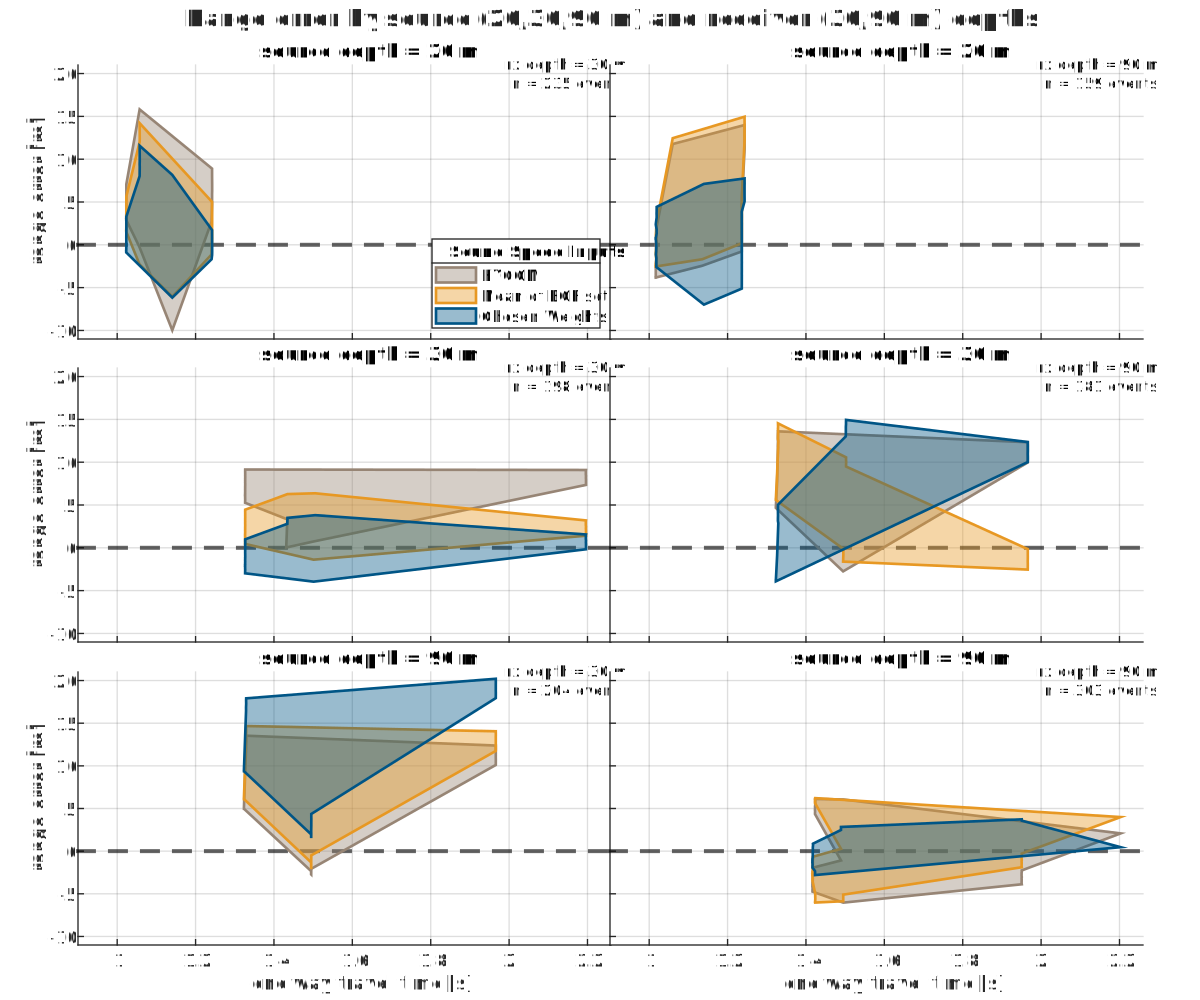
\includegraphics[width=\textwidth]{figs/range-error-owtt-newalgorithm.pdf}
\caption{\label{fig:gvel30}{Caption here.}}
\end{figure}

\FloatBarrier
\subsection{GPS sensor drift}

Systemic GPS drift drives the severe banding found in comparisons of range estimations via both group velocity algorithms, with those bands showing 100\% positive correlation between methods and being a similar size in meters.
Thus, while this thesis is primarily motivated by achieving similar accuracy and precision of GPS, the impressive results from acoustic ranging necessitate a discussion about the limitations of GPS, particularly at polar latitudes.

The ``Global Positioning System Standard Positioning Service Performance Standard'', published by the Department of Defense in Apr 2020 (CITE GPS TECHNICAL STANDARD) claims that well-designed GPS receivers have been achieving a horizontal accuracy of 3 meters and a vertical accuracy of 5 meters, 95\% of the time.
But ``well-designed'' is an ambiguous enough term that obfuscates two confounding factors for high latitude GPS drift\textemdash operational limitations and ionospheric scattering.

% operational
There are two metrics that demonstrate the operational limitations of GPS tracking technologies\textemdash fix rate and positional dilution of precision (PDOP) \citep{swanlund_gps_2016}.
Fix rate looks at the ratio of successful fixes to overall attempts in acquiring a location.
In animal tracking studies in polar latitudes, fix rates have significantly improved in the last twenty years, from as low as 26\% in 1996\citep{moen_effects_1996} to 87.2\% in 2018 \citep{jung_accuracy_2018}.
The latter study showed a precision of 4.3 $\pm$ 4.0 m and an accuracy of 6.0 $\pm$ 4.7 m.
While significant metric to evaluate GPS robustness, accuracy and precision, not the fix rate, explains the severe banding observed; fix rate bias, where various aspects of a landscape can induce bias by impeding the GPS receiver from acquiring its location, is not relevant given the static nature and small time window of ICEX20.

PDOP looks at the effect of satellite geometry on location precision, as satellite orbits are designed to optimize performance for human population density.
A high PDOP value indicates a poor geometric configuration, such as satellites being tightly clustered above a GPS receiver, that limits the reliability of trilateration.
The literature shows correlation between PDOP values and location error \citep{swanlund_gps_2016}.
PDOP is generally thought of as three-dimensional positioning and can be broken down into the horizontal and vertical components, HDOP and VDOP, respectively.
The low elevation angles in polar areas are good for horizontal positioning but are susceptible to poorer vertical positioning.
Overall this contributes to higher noise level in observations than usually seen in most global applications.
The sparse and limited infrastructure in the Arctic make it ideal for satellite-based navigation, with some research proposing new satellite systems to accommodate increased interest in the region \citep{reid_gnss_2016}.

However, both of these metrics are functions of the satellite constellation available to any given GPS receiver.
The Arctic area is beyond the reach of many geostationary satellites, where they are low on the horizon and only visible for brief periods.
Given that their positions are tracked by stations on Earth, and their timing is updated twice a day via atomic clock, a reasonable hypothesis for bands of GPS error are different and/or updated satellite connections.

% ionospheric
The second confounding factor is the ionosphere, the layer of the Earth's atmosphere roughly 80 to 1000 km above the surface that contains a high concentration of ions and free elections. 
In the ionosphere, electromagnetic signals are affected by the total amount of electrons encountered by the signal; the size of the signal delay is dependent on the carrier frequencies.
The normal signal delay creates a GPS error of 5 to 15 meters during the daytime and 1 to 3 meters at night (CITATION).
The literature even references the total amount of electrons encountered by the ``GPS raypath'' as a means of explaining signal fluctuations \citep{themens_nature_2015}.
This variability is observed by seasonal and solar cycle variabilities,\citep{themens_nature_2015} severe ionospheric storms\citep{mitchell_gps_2005}, and auroral activity (increased electron precipitation)\citep{jin_gps_2014,gwal_gps_2011}.
In fact, the \textit{aurora borealis} was observed on multiple nights during ICEX20.

In a humbling twist, at polar latitudes, GNSS systems experience similar operational, technical, and environmental challenges that we observe in underwater acoustic communications; the underwater acoustics community generally seems to ignore these challenges when validating localization and navigation efforts.

Figure \ref{fig:gps-drift-example} highlights the GPS and observed OWTT drift relative to the ice movement for two pairs of modem buoy connections.
The top two panels show GPS drift in both the $x$ and $y$ directions relative to the median $x$ and $y$ distance recorded between the two buoys.
The bottom two panels indicate the GPS drift as $\delta R = \sqrt{\delta x^2 + \delta y^2}$ and temporal drift, $\delta t$, relative to the median OWTT recorded between the two modems.
Here we use the median, not the mean, to be more robust to outliers in the dataset.
The dashed line is scaled by a group velocity of 1440 m/s, such that if there was no GPS drift, all events should exist on the line.

The left hand side of the plot shows the connections between the North and East buoys.
The top shows consistent change in distance with respect to time, as the $\delta X$ measurement trends from 2 to -2 and the $\delta Y$ measurement trends from -1 to 1 meters.
This indicates that the ice movement between the North and East buoys is non-rigid, i.e., they are actually moving relative to each other.
The width of the scatter plot is a decent indicator for the precision of the GPS signal, as it remains consistent across many colors of scattered points, which correspond to similar regions in time.
The idea that these buoys are moving relative to each other is corroborated in the bottom plot, where some events exist on the dashed line indicating correlation between GPS movement and OWTT change.
Some of the offsets between the vertical bands relate to different operational configurations of source and receiver depths.
However, the large majority of events show vertical banding for the same nominal $\delta t$, indicating the amount of GPS drift.

This idea of GPS drift relative to the same OWTT measurements is also indicated by events between the other two buoys, South and West, on the right hand side.
The GPS drift, on the top, shows a point cloud centered around the origin for events four hours and 13 hours after the experiment origin; thus these buoys are moving in a more rigid ice floe.
There is minimal impact by source and receiver depth on the spread of OWTT.
The GPS drift relative to the OWTT, on the bottom, shows a large amount of GPS drift for very little OWTT drift.
The OWTT drift observed here is sensitive to the acoustic scattering, multipath, or environmental microstructure.

These are two subsets of the physical links, they cover all four GPS modem buoys except for Camp.
The GPS at camp, as shown in figure \ref{fig:iceFloe}, is the least accurate due to the human activity and infrastructure occluding the physical puck.
A more comprehensive look at all physical link pairs is in Appendix \ref{app:beacon2beacon}.

\begin{figure}[h!]
	\centering
	\includegraphics[width=\textwidth]{figs/gps-drift-example} 
	\caption[Examination of GPS and modem drift]{A comparison of GPS drift (top) colored by hours since the experiment origin and GPS drift against OWTT spread (bottom) demarcated by source depth and receiver depth. The physical link between North and East are shown on the left; South and West is on the right. }
	\label{fig:gps-drift-example}
\end{figure}

% =========================================================================== %
% =========================================================================== %
\section{\label{sec:4} Discussion}

Range estimation is an essential step of acoustic localization and navigation.
This work solely focuses on mitigating range estimation error via a stochastic prediction of the group velocity, knowing that this can have an outsized benefit on minimizing trilateration error.
We hypothesize and validate that the group velocity, especially for mission durations, is smoothly varying in range and multipath structure, and sensitive to source and receiver depth.
We employ a GPS-tracked experiment to have a ground truth comparison for real-time localization algorithms.

This work, to our knowledge, is the first successful field deployment of a real-time, ray-based acoustic ranging system for underwater navigation.
The methods here demonstrate remarkable ranging accuracy and precision for the Beaufort Lens, an acoustically complex environment.
The \textit{in situ} prediction via BELLHOP balances the tension in simulation fidelity versus capturing the overarching ensemble physics to approximate a local group velocity.

Furthermore, the improved nearest bounce criteria, validated in a high fidelity post-processing pipeline, produces range estimates that rival GPS accuracy and outclass GPS precision, especially at polar latitudes.
It transforms multipath, widely considered as an obstacle for acoustic ranging, into a new information content to refine ranging accuracy.

The scalability of the methods provided here for long-range applications remain to be seen.
Given the NBC algorithm's improvement with increased multipath, its effectiveness is likely only challenged by the valid operational scales of a range independent propagation environment.
Even then, the dominant SSP amongst the variability may very well produce GPS-like accuracy.
The NBC algorithm can be easily be retooled to discriminate between surface and bottom bounces, and employ simple statistical learning or more advanced machine learning techniques to select an appropriate representative group velocity.
Some more advanced vehicle intelligence can toggle use the range uncertainty to toggle between a more conservative group velocity estimate and the NBC, which is intrinsically quite precise.

There are many avenues that this approach can be further refined and tested for field operations.
Amongst them is defining the uncertainty grid for BELLHOP via stochastic or data-driven measures such as the distance traveled by the AUV between ICNN updates or the magnitude of the position corrections by the ICNN.
Another is to entirely remove the seeded range and instead rely on the submerged asset's depth and recorded OWTT to find high probability fields in range, as briefly indicated in Chapter 6.

As the Arctic continues to become more accessible and navigable, safe navigation infrastructure and practices will be increasingly vital for industry, tourism, commercial, and military operations.
This work contributes a new paradigm to embed environmentally adaptive behavior into AUV navigation that has demonstrated success in an acoustically complex and operationally challenging environment.
Thus, we believe that this work enables more accurate range estimation, localization, and/or navigation for any field experiment given known source and receiver depths.

(NEED TO SKIM CONCLUSION FOR MORE MATERIAL)

\FloatBarrier
\section*{Supplementary Figures}

\clearpage
\subsection*{Ice movement during the modem experiment}
\begin{figure}[h!]
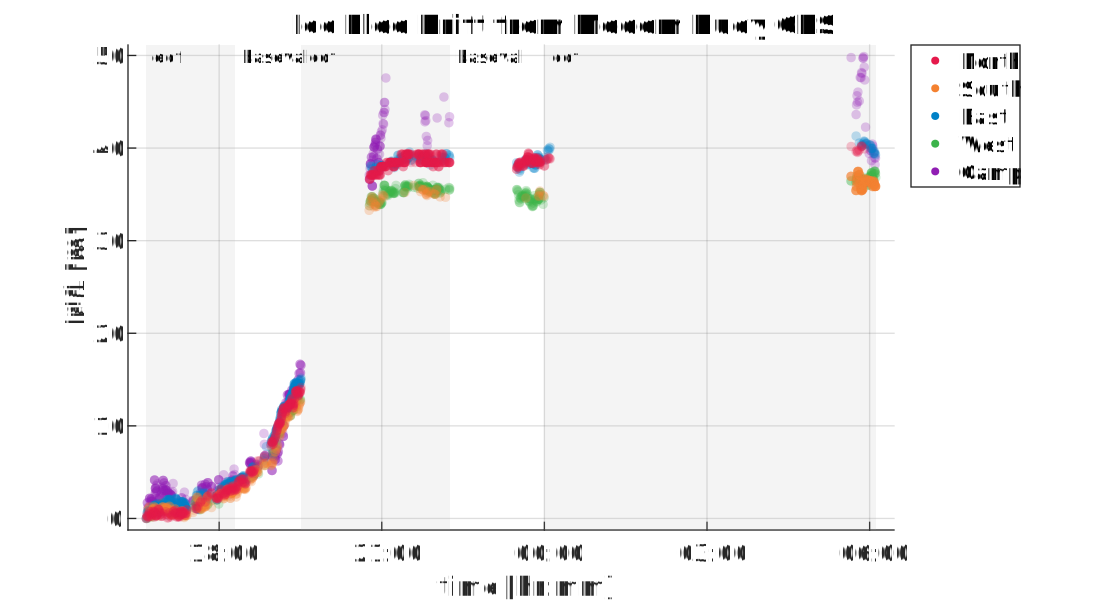
\includegraphics[width=\textwidth]{figs/ice-floe-drift.pdf}
\caption{\label{fig:iceFloeDrift}{Caption here.}}
\end{figure}

\clearpage
\FloatBarrier
\subsection*{Group velocity prediction by source depth}
\begin{figure}[h!]
\includegraphics[width=0.8\textwidth]{figs/SLIDES-gvel-comparison-wdata-20.pdf} \\
\includegraphics[width=0.8\textwidth]{figs/SLIDES-gvel-comparison-wdata-90.pdf}
\end{figure}


% ================================================== %
% \begin{figure}[ht]
% \includegraphics[width=\reprintcolumnwidth]{figsamp.jpg}
% \caption{\label{fig:FIG1}{Caption here.}}

% \raggedright
% {\color{red}
% Note: The only figure formats allowed are the following:
% .pdf, .ps, .eps, or .jpg. Figure files must be named in this fashion:
% Figure\#.xxx, where ``\#'' is the figure number and ``xxx'' is the file format
% (Figure1.eps, Figure2.jpg, Figure3a.ps, Figure3b.ps, etc).
% }

% [For these sample pages we have used only figsamp.jpg for convenience]
% \end{figure}
% ================================================== %





% \subsubsection{Sample subsubsection\label{subsubsec:1}}

% \paragraph{Sample paragraph}Here is text following the paragraph
% heading.
% Here is a figure reference: is shown in Fig.~\ref{fig:FIG1}.



% Normal journal cite: \citep{joursamp1},
%  Book reference \citet{booksamp1},
% Computer language documentation:
% \citep{sampcode2}.

% Every \verb+\citep+  or \verb+\citet{}+ will produce a citation and an entry in the
% bibliography. Every citation must have a matching entry in the
% bibliography
% database file (\verb+\filename.bib+).


% Here is an example of algorithmic:


% \begin{algorithmic}
% \If {$i\geq maxval$}
%     \State $i\gets 0$
% \Else
%     \If {$i+k\leq maxval$}
%         \State $i\gets i+k$
%     \EndIf
% \EndIf
% \end{algorithmic}


\begin{acknowledgments}
This research was supported by the Office of Naval Research and the NDSEG Fellowship. We are grateful to all our collaborators in ICEX20\textemdash Bluefin Robotics, Toby Schneider, Lee Freitag \textemdash 
\end{acknowledgments}

\bibliography{sampbib}